%% Image Processing Project: Feature-Based Image Processing and Reinforcement
%% Learning for CarRacing-v3
%%
%% Compile in Overleaf (recommended) or with a local TeX Live / MiKTeX that
%% includes the IEEEtran package:
%%   latexmk -pdf main.tex
%% or
%%   pdflatex main && bibtex main && pdflatex main && pdflatex main
%%
%% IEEEtran is built into Overleaf and into full TeX Live / MiKTeX distributions.
%% It is NOT shipped in this package.
\documentclass[conference]{IEEEtran}
\usepackage{graphicx}
\usepackage{booktabs}
\usepackage{amsmath}
\usepackage{amssymb}
\usepackage{array}
\usepackage{url}
\usepackage[hidelinks]{hyperref}
\graphicspath{{figures/}}
\setlength{\textfloatsep}{7pt plus 2pt minus 2pt}
\setlength{\floatsep}{7pt plus 2pt minus 2pt}
\setlength{\intextsep}{7pt plus 2pt minus 2pt}

\begin{document}

\title{Image Processing Project: Feature-Based Image Processing and Reinforcement Learning for CarRacing-v3}

\author{\IEEEauthorblockN{Joe}
\IEEEauthorblockA{Student ID: 1103820}}

\maketitle

\begin{abstract}
This project studies an image-processing-centric pipeline for Gymnasium
CarRacing-v3, a continuous-control driving task where the agent observes a
$96\times96$ RGB frame and emits steering, gas, and brake commands. Rather than
training a policy directly on pixels, a deterministic wrapper converts each
frame into an HSV-based road mask, cleans it morphologically, and casts nine
road-distance rays across a calibrated angular fan. The resulting compact
observation is a 16-dimensional vector (nine ray distances, three smoothed
previous actions, speed, a curvature proxy, a front-ray change term, and a
left-right asymmetry term); four consecutive observations are temporally
stacked into a 64-dimensional vector. The same feature pipeline is shared by
two downstream evaluators---a completed Stable-Baselines3 PPO baseline trained
for 500{,}000 steps and a SAC fast-result branch validated at a 400{,}000-step
best checkpoint. The PPO baseline reaches a validated raw reward of
$938.87\pm7.86$ at 500{,}000 steps (best parsed $939.53\pm4.09$ at 480{,}000),
and the SAC branch reaches $938.51\pm4.88$ at 400{,}000. The contribution is
the visual representation; the reinforcement-learning algorithms are evaluation
tools. The method is sample-efficient and promising, but it is not uniformly
robust, and CarRacing-v3 is not claimed to be solved.
\end{abstract}

\begin{IEEEkeywords}
image processing, HSV road mask, ray features, CarRacing-v3, PPO, SAC, feature-based reinforcement learning
\end{IEEEkeywords}

\section{Introduction}

Gymnasium CarRacing-v3 is a compact but demanding continuous-control
benchmark~\cite{ref_gym}. The observation is a $96\times96$ RGB image, and the
action is a three-dimensional continuous vector for steering, gas, and brake. A
policy trained directly on pixels must learn visual perception, local road
geometry, throttle control, and recovery behavior simultaneously. That full
end-to-end problem is attractive as a benchmark, but it is expensive for a
course project where the training budget, hardware time, and debugging time are
limited.

This project takes a narrower and more reproducible path. The core idea is to
keep the reinforcement-learning algorithm standard and move part of the
perception burden into a deterministic image-processing wrapper. Each RGB
observation is cropped, converted to HSV, thresholded into a road mask, cleaned
morphologically, and summarized by nine distance rays. The policy does not
receive the full image; it receives a compact vector describing local road
openness, recent controls, speed, and curvature. The resulting observation is
small enough to train with an MLP policy rather than a convolutional image
policy.

The same compact visual representation is then used as a fixed downstream input
to two standard off-the-shelf learners from Stable-Baselines3~\cite{ref_sb3,
ref_ppo_mod, ref_sac_mod}: a completed PPO~\cite{ref_ppo} baseline and a SAC
fast-result branch~\cite{ref_sac}. Holding the perception layer constant and
varying only the policy optimizer makes the image-processing contribution the
isolated variable of the study.

The design is intentionally conservative. It does not introduce a custom
reinforcement-learning variant, a new neural-network architecture, or a learned
perception module. The wrapper is deterministic image processing, the learners
are unmodified Stable-Baselines3 algorithms, and the final evaluation reloads
saved artifacts from disk. This makes the project auditable: mask thresholds,
ray geometry, action smoothing, reward shaping, algorithm settings,
normalization statistics, and evaluation seeds are all explicit.

The main empirical results are strong but must be read carefully. The PPO
baseline is a fully completed 500{,}000-step run reaching
$938.87\pm7.86$ raw reward (best parsed $939.53\pm4.09$). The SAC branch is a
\emph{partial} fast-result run whose validated number is the 400{,}000-step
best checkpoint ($938.51\pm4.88$); it did not complete 500{,}000 steps. The
PPO/SAC comparison is therefore not compute-equivalent, and SAC is not claimed
to beat PPO. The results support the claim that the compact road-geometry
representation is sample-efficient and promising; they do not support a claim
that the environment is solved or that the method is uniformly robust.

The remainder of the paper defines the environment and problem, describes the
image-processing pipeline and the compact feature representation in detail,
presents the evaluation setup, reports the PPO baseline and SAC fast-result
experiments, analyzes the results, and discusses limitations.

\section{Background and Related Work}

Two broad strategies exist for visual control in CarRacing-v3. The first is
end-to-end pixel control, in which a convolutional policy is trained directly on
the rendered frame and must jointly learn perception and control; this is the
setting most deep reinforcement-learning baselines target~\cite{ref_ppo,
ref_sac}. It is general but sample-hungry and hard to debug, because perception
errors and control errors are entangled inside a single network. The second
strategy, taken here, front-loads perception with deterministic image processing
and leaves only control to the learner. Classical color-space thresholding and
morphological cleanup are long-standing tools for road and free-space
segmentation~\cite{ref_opencv}, and casting distance rays over a free-space mask
is a compact way to encode local geometry without a learned encoder.
Off-the-shelf implementations of PPO and SAC from
Stable-Baselines3~\cite{ref_sb3, ref_ppo_mod, ref_sac_mod} make it possible to
hold the learner fixed and study the representation in isolation. The present
project sits in this second family: the novelty is the hand-designed visual
feature, while the reinforcement-learning algorithms are unmodified evaluators.

\section{Environment and Problem Definition}

CarRacing-v3~\cite{ref_gym} places an agent on a procedurally generated, randomly
laid-out track. At each step the environment renders a top-down $96\times96$ RGB
frame of the area around the car. The action space is continuous and
three-dimensional:
\begin{equation}
a = [\,a_{\text{steer}},\; a_{\text{gas}},\; a_{\text{brake}}\,],
\end{equation}
with $a_{\text{steer}}\in[-1,1]$, $a_{\text{gas}}\in[0,1]$, and
$a_{\text{brake}}\in[0,1]$. The reward is based on progress along the track and
is reduced when the car visits tiles out of order or runs out of time. Tracks
are randomized across episodes, so a successful policy must generalize rather
than memorize a single layout.

Two properties make this a hard visual-control problem. First, the useful
signal (the road and its local geometry) occupies only part of the frame, and
it must be extracted from color and shape rather than given explicitly. Second,
a single episode can look successful for many frames and then fail suddenly
after a sharp turn, an off-road drift, or an unstable recovery. A single
high-scoring video is therefore not sufficient evidence; the project evaluates
saved artifacts on multiple fixed and randomized seed sets and reports mean,
variance, and individual seeds.

The image-processing objective follows directly: convert each rendered frame
into a small, inspectable description of the local road that an MLP policy can
act on quickly and that generalizes across randomized tracks.

\section{Image Processing Pipeline}
\label{sec:pipeline}

The perception wrapper converts a raw RGB frame into a road mask and then into a
set of ray features. Figure~\ref{fig:pipeline} summarizes the six stages.

\begin{figure}[t]
\centering
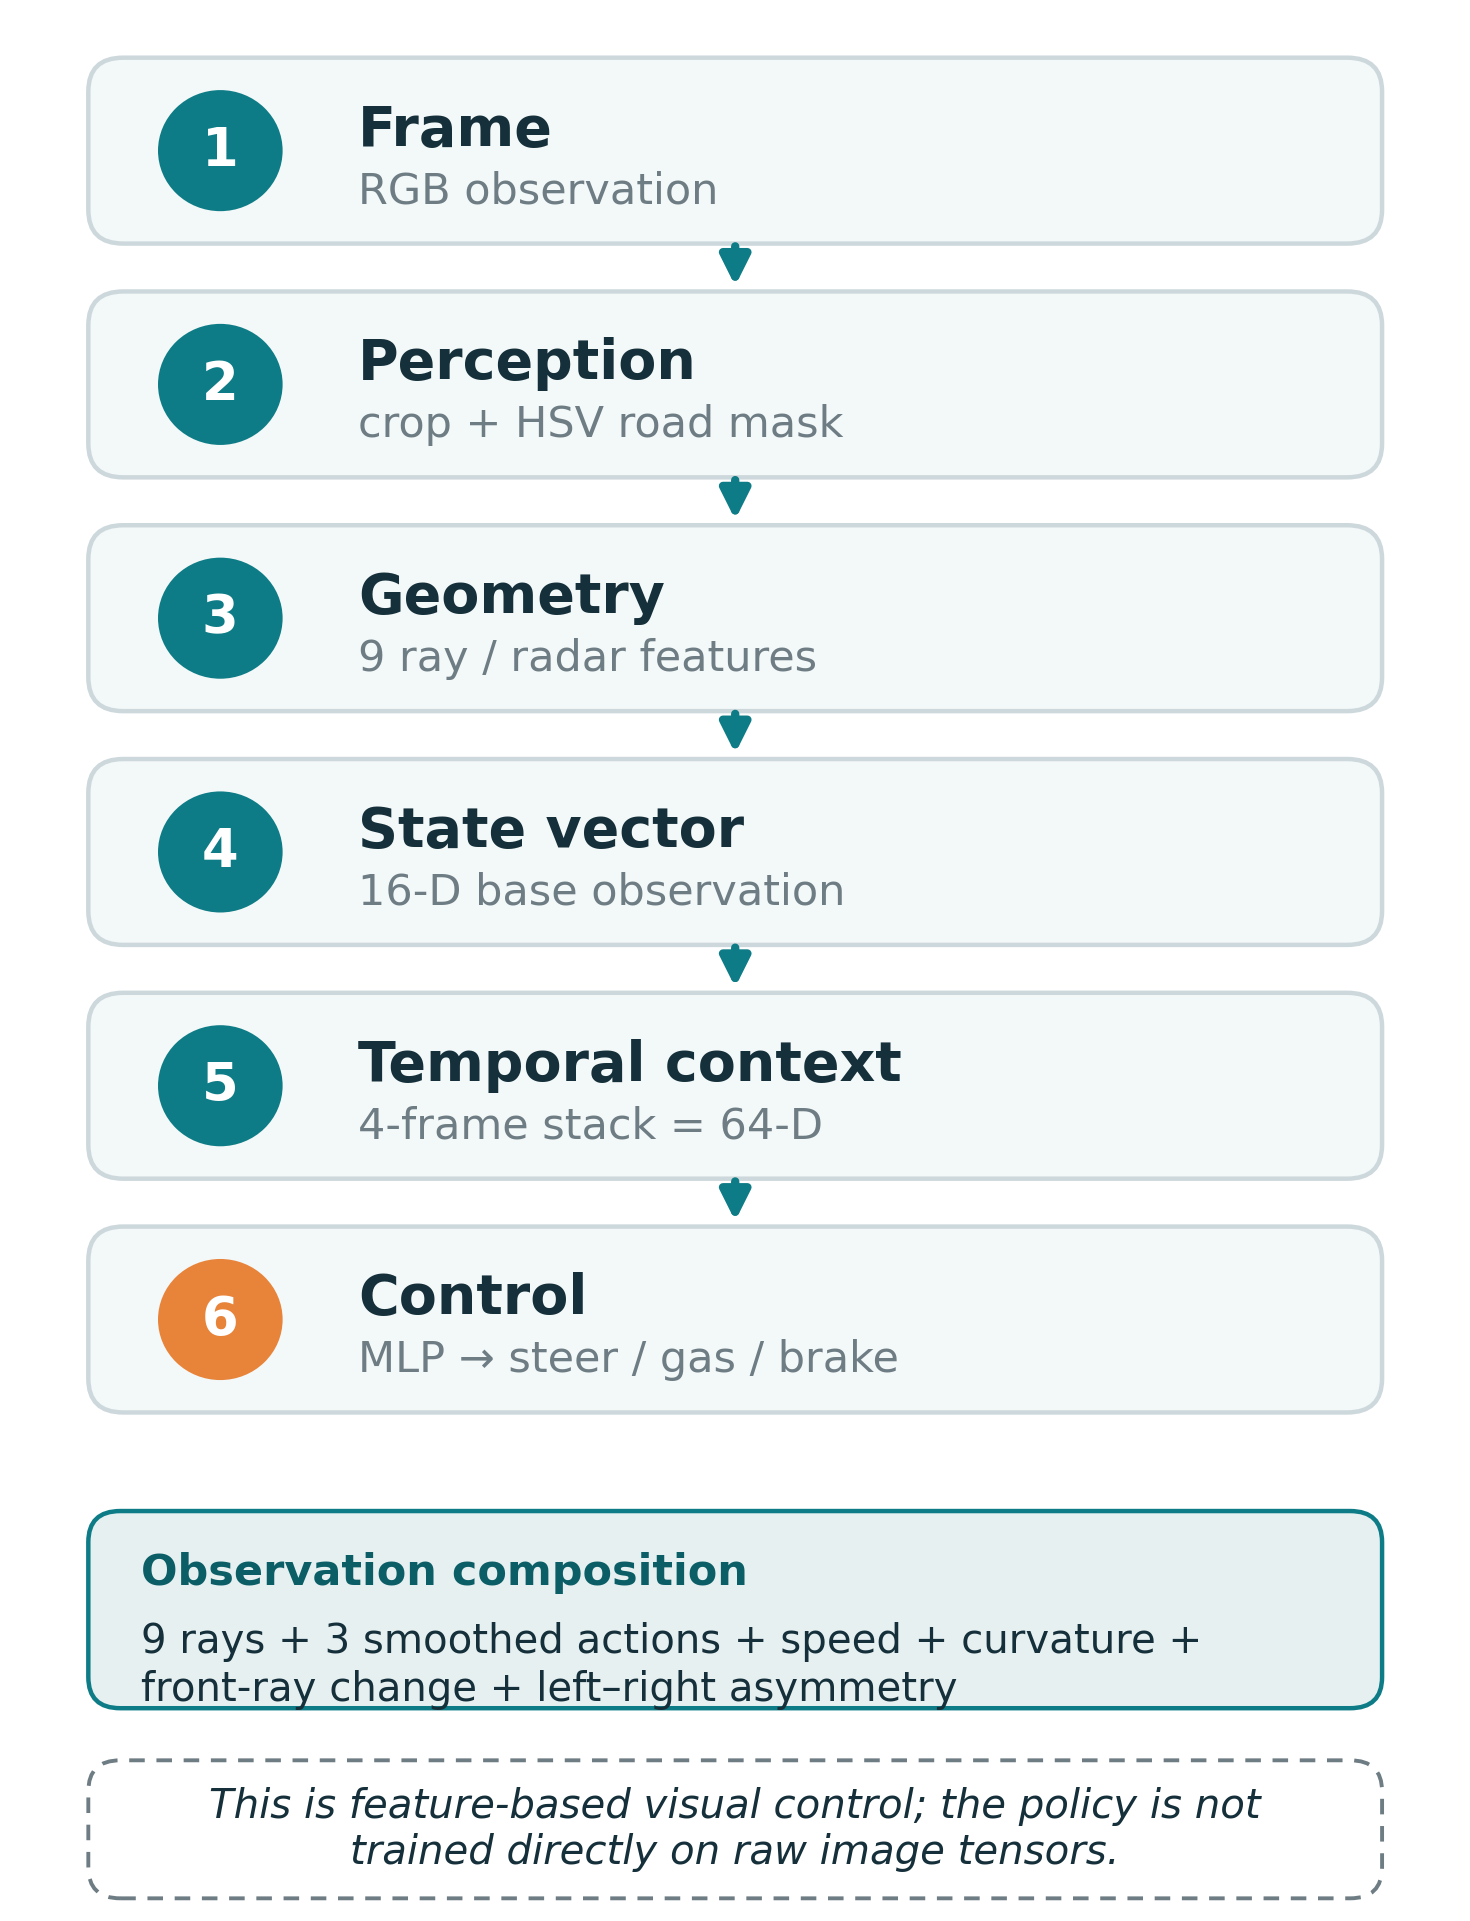
\includegraphics[width=\columnwidth]{feature_pipeline_cards.png}
\caption{Feature-based visual-control pipeline. A rendered RGB frame passes
through six stages: frame (RGB observation), perception (crop and HSV road
mask), geometry (nine ray/radar features), the 16-dimensional base state vector,
temporal context (a four-frame stack, 64-dimensional), and control (an MLP
emitting steering, gas, and brake). The base observation comprises nine rays,
three smoothed actions, speed, curvature, a front-ray change term, and a
left--right asymmetry term. The policy is not trained directly on raw image
tensors.}
\label{fig:pipeline}
\end{figure}

\subsection{Cropping and color conversion}

The lower driving-relevant portion of the frame is retained and converted from
RGB to HSV~\cite{ref_opencv}. Working in HSV separates chromatic information
(road versus grass) from intensity, which makes the road-region threshold more
stable to overall brightness changes than an RGB threshold would be.

\subsection{HSV road-mask extraction}

The road is isolated by removing the grass. In the HSV representation the green
grass occupies a well-defined band, so grass pixels are selected with a fixed
lower and upper bound and the road mask is taken as the bitwise complement:
\begin{equation}
\text{grass}(p) = \mathbb{1}\!\left[\,l \preceq \text{HSV}(p) \preceq u\,\right],
\qquad \text{road} = \neg\,\text{grass},
\end{equation}
with $l=[28,35,35]$ and $u=[92,255,255]$ in OpenCV units
($H\in[0,179]$, $S,V\in[0,255]$)~\cite{ref_opencv}. The hue window $28$--$92$
covers the green range, while the saturation and value floors of $35$ reject very
dark or washed-out pixels that would otherwise be misclassified. Selecting the
grass and complementing it, rather than thresholding the road directly, is more
stable because the grass color is far more uniform than the combined road, curb,
and car pixels.

The raw complement contains speckle and pin-holes, so it is cleaned with a
$3\times3$ morphological opening---an erosion followed by a dilation with the same
structuring element $B$:
\begin{equation}
\text{road} \leftarrow (\text{road} \ominus B) \oplus B .
\end{equation}
The erosion removes isolated bright specks and thin bridges, and the dilation
restores the boundary of the surviving regions, so the dominant road blob keeps
its area while noise is discarded. Finally, a connected-component labeling pass
can restrict the mask to the component containing the car's position, suppressing
detached road-colored patches elsewhere in the frame.

\subsection{Ray casting}

Local road geometry is summarized by nine distance rays cast from a calibrated
origin near the car outward at fixed relative angles spanning a $140^{\circ}$
forward fan:
\begin{equation}
\Theta = [-70,\,-52.5,\,-35,\,-17.5,\,0,\,17.5,\,35,\,52.5,\,70]\text{ deg},
\end{equation}
where $0^{\circ}$ points straight ahead and the sign denotes left ($-$) or right
($+$). Each ray is traced by stepping a point
$\mathbf{p}(t)=\mathbf{p}_0+t\,(\sin\theta,\cos\theta)$ outward in small fixed
increments until it leaves the road mask or reaches a maximum length $L_{\max}$;
the ray's value is the travelled distance normalized to $[0,1]$,
\begin{equation}
r_i = \min\!\big(t_i^{\text{hit}},\,L_{\max}\big)/L_{\max}.
\end{equation}
The nine returns form a one-dimensional profile of how open the road is ahead and
to each side (Fig.~\ref{fig:rays}): a centred peak indicates a clear road ahead,
while an asymmetric profile signals an upcoming bend. To keep the fan informative
at speed, both the angular spread and $L_{\max}$ are modulated by the previous
speed---the fan is gently narrowed (``squeezed'') and lengthened when the car is
fast, giving a tighter, longer look-ahead, and widened when it is slow.

\begin{figure}[t]
\centering
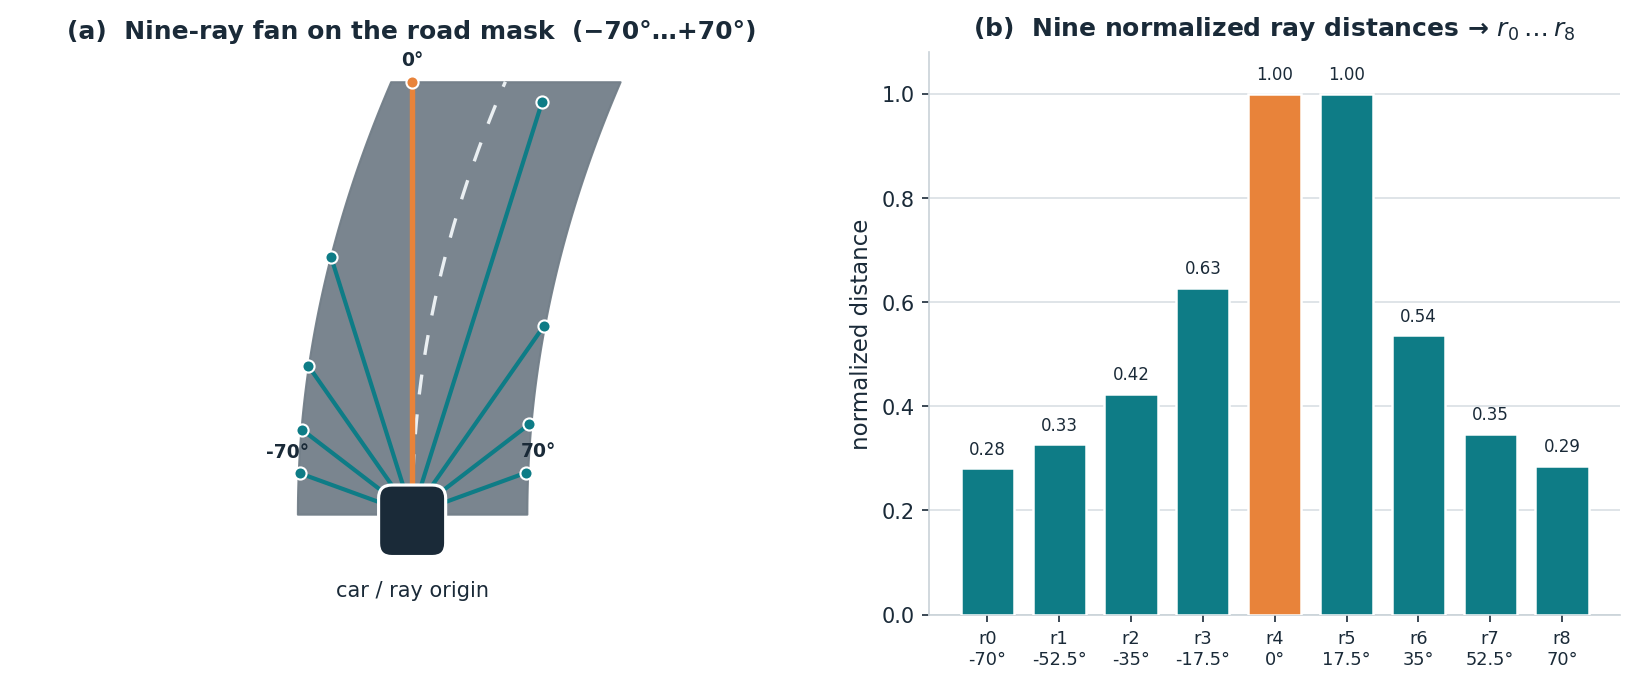
\includegraphics[width=\columnwidth]{ray_fan_schematic.png}
\caption{Ray-feature extraction. (a) Nine rays are cast across the calibrated
$-70^{\circ}$ to $+70^{\circ}$ fan and stop at the road-mask boundary, with the
centre ray ($0^{\circ}$) highlighted. (b) The travelled distances, normalized to
$[0,1]$, become the nine ray components $r_0\dots r_8$ of the observation. The
asymmetric profile shown here encodes a road bending to the right.}
\label{fig:rays}
\end{figure}

\subsection{From mask and rays to a compact observation}

The ray profile is the backbone of the observation, but it is augmented with
control- and dynamics-oriented terms so the policy has enough state to act
smoothly and recover. The curvature proxy is derived from the asymmetry between
the left and right ray groups and the central ray depth; the front-ray change
term measures the difference between the current central ray and its previous
value, giving a local derivative of forward openness; and the left-right
asymmetry term summarizes the bias of the road to one side. These are described
in detail in Section~\ref{sec:features}.

\section{Feature Representation Design}
\label{sec:features}

\subsection{Base observation vector}

The base observation is a 16-dimensional vector:
\begin{equation}
o_t = [\,r_0,\dots,r_8,\; \tilde a_{t-1},\; v_t,\; \kappa_t,\; \Delta f_t,\; \alpha_t\,],
\label{eq:obs}
\end{equation}
where $r_0,\dots,r_8$ are the nine normalized ray distances;
$\tilde a_{t-1}\in\mathbb{R}^3$ are three smoothed previous action terms;
$v_t$ is the speed; $\kappa_t$ is the curvature proxy; $\Delta f_t$ is the
front-ray change term; and $\alpha_t$ is the left-right asymmetry term. The
composition is summarized in Table~\ref{tab:obs}.

\begin{table}[t]
\caption{Composition of the 16-dimensional base observation.}
\label{tab:obs}
\centering
\small
\begin{tabular}{rll}
\toprule
Index & Component & Source \\
\midrule
0--8   & 9 ray distances $r_0\dots r_8$ & ray casting on road mask \\
9--11  & 3 smoothed previous actions $\tilde a_{t-1}$ & action history \\
12     & speed $v_t$ & environment state \\
13     & curvature proxy $\kappa_t$ & ray-group asymmetry \\
14     & front-ray change $\Delta f_t$ & central ray derivative \\
15     & left-right asymmetry $\alpha_t$ & ray-group means \\
\bottomrule
\end{tabular}
\end{table}

The curvature proxy is active only when the forward road is judged to be
present (the mean of the central forward rays exceeds a small threshold),
which prevents the curvature estimate from responding to off-road noise.

Each augmenting term carries a specific control role. The three smoothed previous
actions $\tilde a_{t-1}$ give the policy access to its own recent commands, which
discourages jittery steering and lets a maneuver continue smoothly. The speed
$v_t$ disambiguates otherwise identical ray profiles that demand different
throttle or braking. The curvature proxy $\kappa_t$ and the left--right asymmetry
$\alpha_t$ pre-compute the direction and magnitude of the turn from the ray
groups, so the network need not re-derive them. The front-ray change $\Delta f_t$
is a one-step derivative of forward openness that gives early warning of an
approaching edge before the absolute distance becomes small.

\subsection{Temporal stacking}

A single frame's observation is instantaneous and cannot express motion.
Following standard practice, $N=4$ consecutive observations are stacked to
form the policy input:
\begin{equation}
s_t = [\,o_{t-3},\; o_{t-2},\; o_{t-1},\; o_t\,] \in \mathbb{R}^{64}.
\end{equation}
The stacked $64$-dimensional vector carries short-horizon dynamics (velocity of
the rays, change in curvature, action momentum) while remaining far smaller and
more inspectable than a stack of raw image tensors.

\subsection{Shared representation across algorithms}

A central design decision is that the perception layer is \emph{held constant}.
The 16-dimensional base observation and the 64-dimensional stacked observation
are identical for both downstream evaluators. PPO and SAC therefore see exactly
the same visual feature stream; the only difference between the two experiments
is the policy optimization algorithm. This isolates the image-processing
contribution as the common variable and makes any behavioral difference
attributable to the learner rather than to the representation.

\subsection{Reward and action shaping}

The environment's raw reward (track progress) is the headline metric and is the
quantity reported in all results. During training only, a shaped reward combines
the raw reward with auxiliary terms (for example on-road incentives and
anti-stagnation terms) to stabilize early learning. Shaped reward is a training
aid; all reported numbers are raw rewards. The action is also smoothed so that
the policy emits continuous, non-jittery commands.

\section{Reinforcement Learning Evaluation Setup}

Both learners are off-the-shelf Stable-Baselines3 algorithms with MLP
policies~\cite{ref_sb3, ref_ppo_mod, ref_sac_mod}. No algorithm is modified.
The wrapper-defined compact observation (Section~\ref{sec:features}) is wrapped
in a vectorized environment with observation normalization
(\texttt{VecNormalize}). Checkpoint-based evaluation callbacks record the best
mean reward during training and save the matching model and normalization
statistics.

\subsection{Checkpoint and reload logic}

Evaluation is artifact-driven. At evaluation time, the saved model parameters
are restored from a saved checkpoint and the saved \texttt{VecNormalize}
statistics are reloaded so that observation normalization at evaluation matches
training. The model is reloaded without reattaching the training environment,
which keeps the evaluation seed schedule fixed and prevents it from being
overwritten during reload. For the SAC fast-result branch, the saved
400{,}000-step checkpoint is used as the fast-result best checkpoint.

\subsection{Evidence hierarchy}

Headline metrics are parsed from the training logs and the validated best
checkpoints. A secondary tier of evidence is computed from saved notebook
outputs on a fixed multi-seed evaluation set and a randomized multi-seed
evaluation set, with a bootstrap confidence interval. These secondary values
are reported separately and are never confused with the log-validated headline
metrics.

\section{PPO Baseline Experiment}

The PPO baseline~\cite{ref_ppo} is a completed 500{,}000-step run. Throughput
was approximately 40 frames per second (elapsed roughly 12{,}417 seconds). The
final evaluation at 500{,}000 steps reaches a raw reward of
$938.87\pm7.86$, and the best parsed checkpoint is $939.53\pm4.09$ at
480{,}000 steps. The full per-checkpoint curve is reported in the Appendix
(Table~\ref{tab:ppo}).

The curve shows the expected noisy climb through the middle of training,
followed by a clear stabilization into the low-930s to low-940s band over the
final checkpoints. The last observed training step was 501{,}760, confirming
that the run reached the full budget.

\section{SAC Fast-Result Branch}

The SAC fast-result branch~\cite{ref_sac} is a \emph{partial} run. Its
validated result is the 400{,}000-step best checkpoint, which reaches a raw
reward of $938.51\pm4.88$. The last observed training step was 418{,}697
(roughly 82\% of 500{,}000), and there is no evaluation checkpoint after
400{,}000 in the provided log; steps beyond 400{,}000 are therefore not treated
as a validated best result. Throughput was approximately 36 frames per second
(elapsed roughly 11{,}400 seconds). Early stopping reflects Colab runtime
limits and the fast-result intent of the branch. The full per-checkpoint curve
is reported in the Appendix (Table~\ref{tab:sac}).

\section{Results and Analysis}

\begin{figure}[t]
\centering
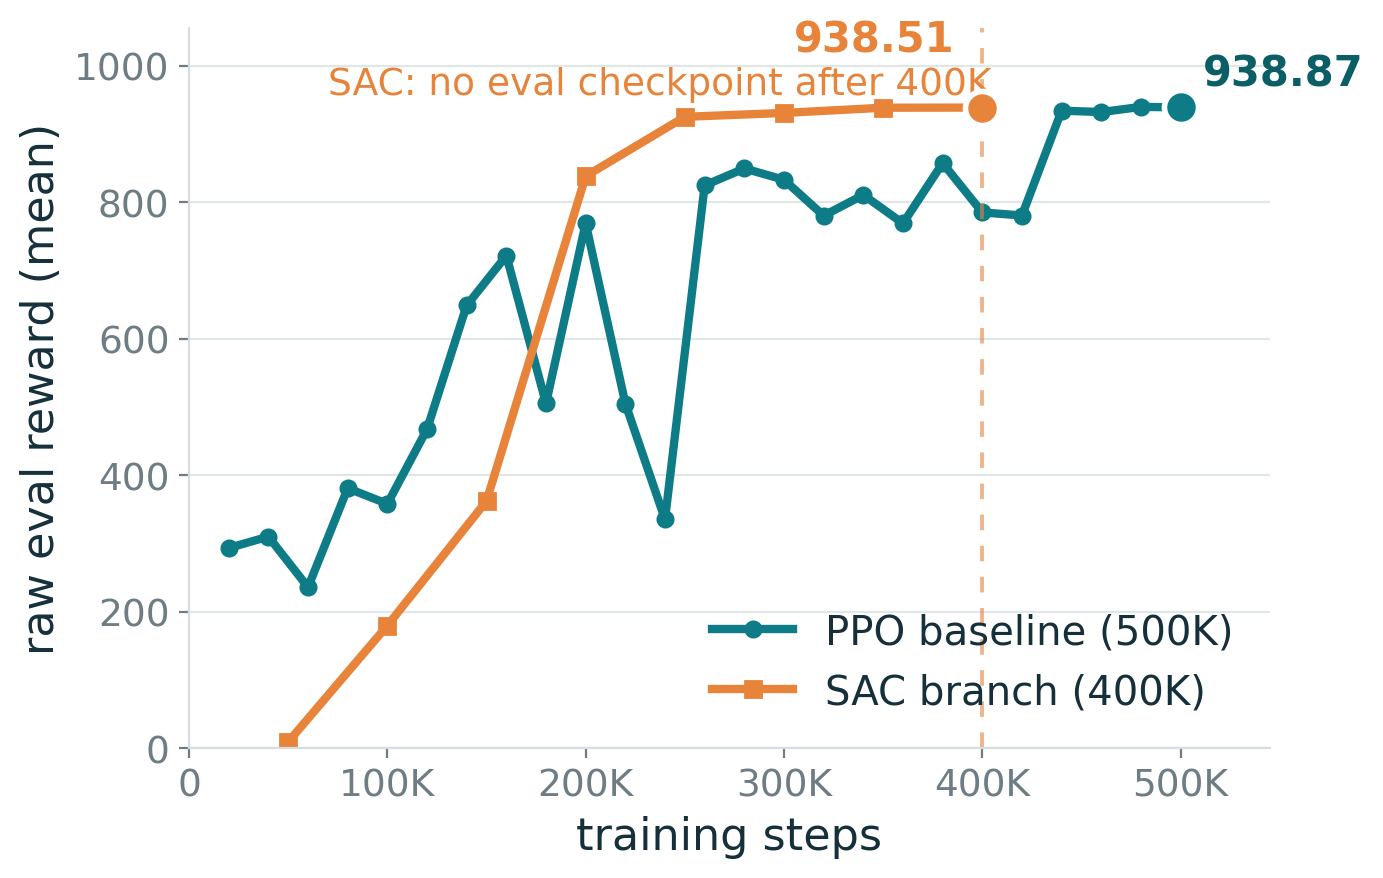
\includegraphics[width=\columnwidth]{training_curve_ppo_sac.png}
\caption{Training curves of the PPO baseline and the SAC fast-result branch,
plotted from the checkpoint tables. SAC stops at the validated 400{,}000-step
checkpoint.}
\label{fig:curve}
\end{figure}

\subsection{Headline comparison}

Table~\ref{tab:headline} summarizes the headline comparison. Both learners reach
the low-930s to low-940s band on the shared compact representation, which is the
main qualitative finding: the same image-processing-derived feature stream
supports strong driving behavior under two different off-the-shelf policy
optimizers.

\begin{table}[t]
\caption{Headline comparison. PPO is a completed 500K baseline; SAC is a partial
400K best-checkpoint fast-result branch. The comparison is not compute-equivalent.}
\label{tab:headline}
\centering
\small
\begin{tabular}{l p{0.30\columnwidth} p{0.34\columnwidth}}
\toprule
Branch & Status & Validated eval \\
\midrule
PPO baseline & Completed 500K baseline & $938.87\pm7.86$ @ 500K; best $939.53\pm4.09$ @ 480K \\
SAC branch & Partial 400K best checkpoint & $938.51\pm4.88$ @ 400K \\
\bottomrule
\end{tabular}
\end{table}

\subsection{Checkpoint and compute budget}

Figure~\ref{fig:curve} shows the two training curves. PPO climbs noisily and
then stabilizes; SAC converges faster in raw-reward terms within its partial
budget. Because the two runs differ in validated budget (500K versus 400K),
throughput, and total elapsed time, the curves are descriptive and not a
controlled ablation. The compute budget is disclosed in Table~\ref{tab:compute}.

\begin{table}[t]
\caption{Compute and budget disclosure.}
\label{tab:compute}
\centering
\small
\begin{tabular}{lll}
\toprule
Branch & Validated budget & Throughput / elapsed \\
\midrule
PPO baseline & 500{,}000 (completed) & $\sim$40 fps / 12{,}417 s \\
SAC branch & 400{,}000 (partial) & $\sim$36 fps / 11{,}400 s \\
\bottomrule
\end{tabular}
\end{table}

\subsection{Secondary generalization evidence}

Beyond the log-validated headline metrics, saved notebook outputs provide
secondary generalization evidence on a fixed multi-seed evaluation set, a
randomized multi-seed evaluation set, and a bootstrap confidence interval. These
values are summarized in Figure~\ref{fig:gen} and Table~\ref{tab:gen} and are
explicitly secondary: they are computed from saved notebook outputs and must not
be read as log-validated headline numbers.

\begin{figure}[t]
\centering
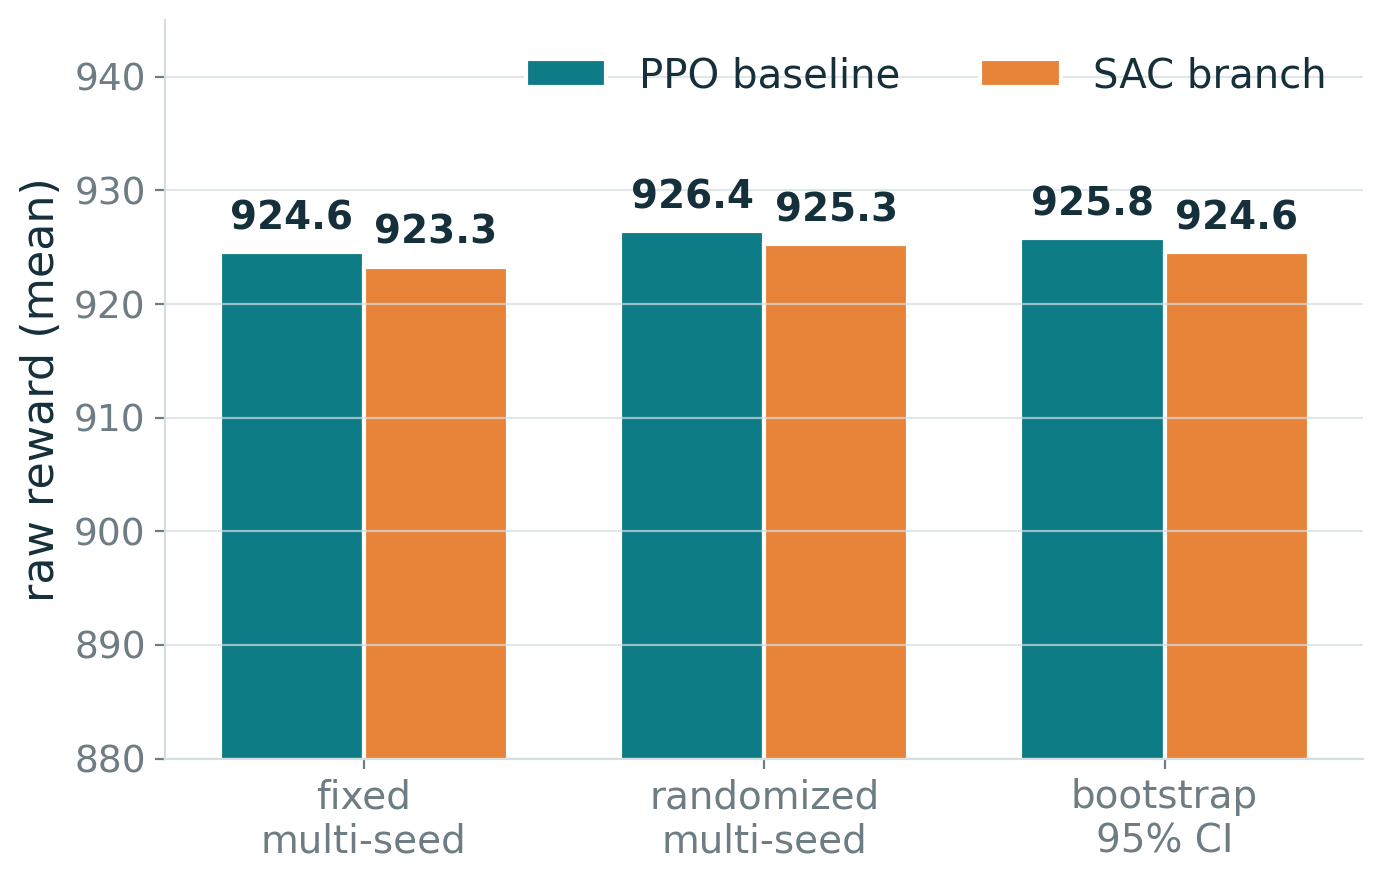
\includegraphics[width=\columnwidth]{generalization_summary.png}
\caption{Secondary generalization evidence from saved notebook outputs (fixed
multi-seed set, randomized multi-seed set, and bootstrap confidence interval).
This is notebook-output evidence, distinct from the log-validated headline
metrics.}
\label{fig:gen}
\end{figure}

Both branches land in the mid-920s on the held-out seed sets---a few points below
the best single checkpoints in Table~\ref{tab:headline}, as expected when
averaging over harder randomized layouts---and the bootstrap confidence intervals
are narrow, which indicates the mean behavior is stable even though individual
seeds vary.

\begin{table}[t]
\caption{Secondary generalization evidence (saved notebook outputs), on a fixed
multi-seed set, a randomized multi-seed set, and a bootstrap 95\% confidence
interval. Reported separately from the log-validated headline metrics.}
\label{tab:gen}
\centering
\small
\begin{tabular}{l l r}
\toprule
Branch & Split & Mean $\pm$ std \\
\midrule
PPO baseline & fixed seeds  & $924.6\pm6.8$ \\
PPO baseline & random seeds & $926.4\pm7.3$ \\
PPO baseline & bootstrap CI & $925.8\;[922.2,929.0]$ \\
SAC branch   & fixed seeds  & $923.3\pm7.7$ \\
SAC branch   & random seeds & $925.3\pm8.2$ \\
SAC branch   & bootstrap CI & $924.6\;[920.7,928.2]$ \\
\bottomrule
\end{tabular}
\end{table}

\section{Discussion and Limitations}

The central result is that an image-processing-derived compact representation,
rather than raw pixels, can support strong driving behavior with off-the-shelf
learners and an MLP policy. Holding the representation constant across PPO and
SAC isolates the perception contribution: both learners reach the same reward
band on the same feature stream, which is consistent with the hypothesis that
the representation---not the learner---is doing the heavy lifting in this
setting.

Several limitations bound these conclusions. First, the SAC result is a partial
fast-result branch validated only at the 400{,}000-step checkpoint; it did not
complete 500{,}000 steps, so the PPO/SAC comparison is not compute-equivalent
and SAC is not claimed to beat PPO. Second, no raw image-input CNN policy was
trained in this submission, so the compact representation is not benchmarked
against a pixel baseline here. Third, HSV-based road-mask extraction depends on
color appearance and can be sensitive to rendering or track-art changes; the
method is not claimed to be uniformly robust. Fourth, the project does not claim
that CarRacing-v3 is solved.

\emph{Failure modes.} The aggregate rewards still hide behavioral limitations.
Even when an episode receives a high raw reward, the driving behavior may include
unstable recovery after sharp turns, brief grass excursions, or moments where
the road mask and ray fan do not anticipate the next turn early enough.
Therefore, the limitation clips should be interpreted as qualitative examples of
remaining control and perception weaknesses, not necessarily as catastrophic
low-reward failures. This long-tail behavior is the main reason the method is
described as promising rather than uniformly robust, and it is why results are
reported as multi-seed statistics rather than a single best episode.

\section{Conclusion}

This project presented an image-processing-centric pipeline for CarRacing-v3 in
which rendered RGB frames are converted into a compact, inspectable road-mask
ray/radar feature representation. The representation---a 16-dimensional base
observation temporally stacked into a 64-dimensional vector---is shared by a
completed PPO baseline ($938.87\pm7.86$ at 500{,}000 steps; best parsed
$939.53\pm4.09$) and a SAC fast-result branch ($938.51\pm4.88$ at the 400{,}000
best checkpoint). The reinforcement-learning algorithms are unmodified
Stable-Baselines3 evaluators; the contribution is the visual representation.
The method is sample-efficient and promising, but the SAC result is partial,
the PPO/SAC comparison is not compute-equivalent, and CarRacing-v3 is not
claimed to be solved. Future work includes matched-budget multi-seed runs, a
raw-pixel baseline, and systematic ablation of the perception stages.

\appendix

\section{Full evaluation checkpoint tables}
\label{app:tables}
Tables~\ref{tab:ppo} and~\ref{tab:sac} list the complete per-checkpoint
evaluation curves for the two branches, parsed from the training logs and
summarized in the main text.

\begin{table}[t]
\caption{PPO baseline: raw reward (mean $\pm$ std) at evaluation checkpoints,
parsed from the training log.}
\label{tab:ppo}
\centering
\small
\begin{tabular}{rr@{\hspace{6pt}}r@{\hspace{6pt}}r}
\toprule
Step & Reward & Step & Reward \\
\midrule
20{,}000  & 293.54$\pm$146.56 & 280{,}000 & 849.36$\pm$173.34 \\
40{,}000  & 310.22$\pm$89.79  & 300{,}000 & 832.78$\pm$204.18 \\
60{,}000  & 236.05$\pm$79.57  & 320{,}000 & 780.22$\pm$211.17 \\
80{,}000  & 381.07$\pm$69.73  & 340{,}000 & 810.58$\pm$233.17 \\
100{,}000 & 358.19$\pm$132.66 & 360{,}000 & 768.91$\pm$211.34 \\
120{,}000 & 467.53$\pm$211.29 & 380{,}000 & 857.28$\pm$104.10 \\
140{,}000 & 648.81$\pm$243.53 & 400{,}000 & 784.98$\pm$178.68 \\
160{,}000 & 721.70$\pm$135.85 & 420{,}000 & 780.46$\pm$317.26 \\
180{,}000 & 505.19$\pm$296.11 & 440{,}000 & 934.05$\pm$6.67 \\
200{,}000 & 769.12$\pm$223.36 & 460{,}000 & 931.94$\pm$2.33 \\
220{,}000 & 505.04$\pm$355.49 & 480{,}000 & 939.53$\pm$4.09 \\
240{,}000 & 335.40$\pm$109.84 & 500{,}000 & 938.87$\pm$7.86 \\
260{,}000 & 824.59$\pm$182.66 & & \\
\bottomrule
\end{tabular}
\end{table}

\begin{table}[t]
\caption{SAC branch: raw reward (mean $\pm$ std) at evaluation checkpoints,
parsed from the training log. No checkpoint exists after 400{,}000.}
\label{tab:sac}
\centering
\small
\begin{tabular}{rl}
\toprule
Step & Reward (mean $\pm$ std) \\
\midrule
50{,}000  & 9.67$\pm$8.98 \\
100{,}000 & 179.94$\pm$28.69 \\
150{,}000 & 362.34$\pm$53.22 \\
200{,}000 & 838.10$\pm$151.24 \\
250{,}000 & 924.99$\pm$4.55 \\
300{,}000 & 930.68$\pm$6.09 \\
350{,}000 & 938.33$\pm$2.42 \\
400{,}000 & 938.51$\pm$4.88 \\
\bottomrule
\end{tabular}
\end{table}

\section{Reproducibility note}
The notebooks are kept in safe report/evaluation mode
(\texttt{SAFE\_MODE}, \texttt{REPORT\_ONLY}, \texttt{EVAL\_ONLY} enabled and
training disabled by default). Headline metrics are parsed from the training
logs and validated best checkpoints. The full checkpoint tables
(Tables~\ref{tab:ppo} and \ref{tab:sac}) are the primary numerical evidence;
the secondary generalization evidence is computed from saved notebook outputs.

\bibliographystyle{IEEEtran}
\bibliography{references}

\end{document}
